\documentclass[conference]{IEEEtran}
\usepackage[T1]{fontenc}
\usepackage{graphicx}
\usepackage{booktabs}
\usepackage{amsmath}
\usepackage{url}
\usepackage{xcolor}
\usepackage[hidelinks]{hyperref}

\begin{document}

\title{Small Open LLM Judges Do Not Follow a Reversed Criterion:\\
A Pair-Level Diagnosis of ``Which Response Is Worse?'' in 0.5--1.7B Models}

\author{\IEEEauthorblockN{Autonomous Research Agent (Claude), on behalf of @pranavnandyalam}
\IEEEauthorblockA{Produced by an autonomous AI agent (Claude) on behalf of @pranavnandyalam. Not peer reviewed.}}

\maketitle

% All numbers in this paper are copied from ../RESULTS.md, ../results/analysis.md, ../results/analysis.json,
% ../results/projection.json, ../results/splits.json, ../results/models.md and figures/paper_stats.json
% (the last is generated by make_figures.py from ../results/raw_*.json).

\begin{abstract}
Small open language models are attractive as cheap pairwise judges, but it is unclear whether they condition
their verdict on the stated criterion at all. We test this by negating the criterion: each pair is judged under
``Which response is better?'' and ``Which response is worse?'', with both presentation orders, giving four
judgments per pair. A pair-level taxonomy separates correct reversal from position-locking (same letter in all
four judgments) and criterion-blindness (same response under both criteria). We evaluate
Qwen2.5-0.5B/1.5B-Instruct and Qwen3-0.6B/1.7B (no thinking, next-token A-vs-B logit readout, CPU) on 300
RewardBench pairs. Correct reversal occurs in 0, 0, 0 and 1 of 300 pairs, respectively. The pre-registered
position-locking hypothesis is supported for the two smallest judges: position-locked shares among
non-correct-reversal pairs are 1.000 (Qwen2.5-0.5B, which answers ``A'' on all 1600 passes) and 0.890
(Qwen3-0.6B, 95\% CI [0.857, 0.927]). The larger judge of each family is less position-locked (0.710 and
0.431; exploratory) but this is replaced by inconsistent behavior, not by correct reversal. The pre-registered hypothesis
that the conditional flip rate rises with size is inconclusive: too few pairs are judged correctly under
``better'' in both orders for the smallest judges (n=0 and n=15), and all conditional flip rates are at most 0.008 (unconditional at most 0.040).
A length control (``Which response is longer?'') is likewise not followed above the random-judge level by any
judge. These are negative results for four models, one benchmark and one prompt format.
\end{abstract}

\begin{IEEEkeywords}
LLM-as-a-judge, pairwise evaluation, position bias, criterion negation, small language models, negative result
\end{IEEEkeywords}

\section{Introduction}
Pairwise LLM judges are widely used to compare model outputs~\cite{zheng2023judging}, and their position bias
is well documented~\cite{wang2023fair,shi2025judging}. Small open models (below 2B parameters) are attractive
judges because they run on commodity CPUs, and recent work evaluates Qwen3 models as small as 0.6B as judges on
RewardBench~\cite{jayarao2025explicit}. A basic precondition for any judge is that its verdict depends on the
criterion it is asked about. Accuracy on a ``which is better?'' prompt cannot establish this: a judge can score
above zero for reasons unrelated to the criterion, and an order-swap test detects position bias but cannot tell
whether the judge reads the question.

We probe criterion conditioning by negation. If a judge prefers the chosen response under ``better'', it should
prefer the rejected one under ``worse''. Asking both questions in both presentation orders gives four judgments
per pair, which is enough to distinguish a judge that reverses correctly from one that always outputs the same
letter and from one that always picks the same response regardless of the criterion.

\textbf{Contributions.}
\begin{enumerate}
\item A four-judgment, pair-level taxonomy (correct reversal, position-locked, criterion-blind,
reversed-consistent, other) with analytic random-judge and always-A reference rows, which separates
position-locking from criterion-blindness (Section~\ref{sec:method}).
\item A pre-registered evaluation of four sub-2B open judges from two families (Qwen2.5, Qwen3) on 300
RewardBench pairs with pinned model and data revisions (Section~\ref{sec:setup}).
\item A negative result: correct reversal is essentially absent (0, 0, 0, 1 of 300 pairs); the two smallest
judges are dominated by position-locking; the pre-registered size-trend hypothesis is inconclusive
(Section~\ref{sec:results}).
\item Exploratory controls suggesting the failure is not specific to negation: a second negated wording and a
``which is longer?'' control are also not followed; the length control is uninformative for the
position-locked judges, which cannot follow any criterion (Section~\ref{sec:results}).
\end{enumerate}

\section{Related Work}
\textbf{Position and order bias.} Zheng et al.~\cite{zheng2023judging} report position and verbosity bias in
LLM judges; Wang et al.~\cite{wang2023fair} show that rankings can be changed by reordering candidates and
propose balanced-position calibration; Shi et al.~\cite{shi2025judging} study position bias systematically
across 15 judges. Mukherjee and Sitaram~\cite{mukherjee2026opening} evaluate 64 open-weight judges and report
that, on LLMBar~\cite{zeng2024llmbar}, verdicts of 50 judges agree with human labels only 0.456 of the time even
after averaging both orders. These works measure order effects under a fixed criterion; they do not negate the
criterion.

\textbf{Criterion and goal reversal.} Closest to this work, GRP~\cite{song2025grp} asks judges which answer is
\emph{worse} and recovers preferences by elimination, reporting improved consistency for GPT-4o and
Claude-3.5-Sonnet on JudgeBench. We use the same negated question, but as a diagnostic of small open judges
rather than as a prompting method for strong closed ones. Bagaria et al.~\cite{bagaria2026rubric} perturb
rubric-based pointwise judging by reversing either the response or the rubric criterion, with
Qwen2.5-7B-Instruct as the only judge; they report desired verdict flips of 37.7\% under response reversal and
16.8\% and 32.2\% (for two candidate models) under criterion reversal. They do not vary judge size and do not
use pairwise order swaps. Prompt-Reverse Inconsistency (PRIN)~\cite{ahn2025prin} contrasts ``which answers are
correct?'' with ``which are incorrect?'' in multiple-choice settings with models of 8B parameters and larger.
JudgeSense~\cite{bellibatlu2026judgesense} measures judge sensitivity to prompt rewording more broadly.

\textbf{Negation in language models.} Kassner and Sch\"utze~\cite{kassner2020negated} show that pretrained
LMs often fail to distinguish negated from affirmative probes, and Jang et al.~\cite{jang2022negated} report
that larger LMs can perform worse on negated prompts.

\textbf{Difference from prior work.} In a limited arXiv and web scan (Semantic Scholar was rate-limited and not
used), we did not find a study of pairwise criterion negation in open judges below 2B parameters that
separates position-locking from criterion-blindness at the pair level. Because small-judge position bias and
below-chance small judges are already reported~\cite{mukherjee2026opening}, our claim is narrow: the
negation-based taxonomy applied to four sub-2B judges, and the resulting negative result. We do not claim to be
first.

\section{Method}\label{sec:method}
\textbf{Prompt.} Each judgment uses the model's chat template with a single user turn containing the user
request, ``[Response A]'' and ``[Response B]'', a question, and ``Answer with a single letter: A or B.''
The questions are: \emph{better} (``Which response is better?''), \emph{W1} (``Which response is worse?'',
primary negation), \emph{W2} (``Which response should be rejected?'', secondary), and \emph{length} (``Which
response is longer?'', control). For Qwen3 we pass \texttt{enable\_thinking=False}.

\textbf{Readout.} We run one forward pass and compare the next-token logits of the single tokens ``A'' and
``B'' (token ids verified per tokenizer); the verdict is the letter with the higher logit. We also record the
probability mass on \{``A'', `` A'', ``B'', `` B''\} as a format-compliance measure. Inference is
deterministic.

\textbf{Four judgments per pair.} For each RewardBench pair (chosen $C$, rejected $R$) we ask \emph{better}
and W1, each with $C$ shown as A (order \emph{cf}) and with $R$ shown as A (order \emph{rf}). Each letter is
mapped back to $C$ or $R$.

\textbf{Taxonomy.} Each pair receives the first matching category:
(1)~\emph{correct reversal}: $C$ in both orders under \emph{better} and $R$ in both orders under W1;
(2)~\emph{position-locked}: the same letter in all four judgments;
(3)~\emph{criterion-blind}: the same response in all four judgments;
(4)~\emph{reversed-consistent}: $R$ in both orders under \emph{better} and $C$ in both orders under W1;
(5)~\emph{other}. Under a uniformly random judge the 16 outcomes are equally likely, giving shares 1/16, 2/16,
2/16, 1/16 and 10/16.

\textbf{Metrics.} \emph{Position-consistent accuracy} is the share of pairs with $C$ chosen in both orders
under \emph{better}; these pairs form the conditioning subset of size $n_\mathrm{cond}$. The
\emph{conditional flip rate} is the share of the conditioning subset for which W1 selects $R$ in both orders.
The \emph{unconditional flip rate} $u$ is the share of all pairs for which W1 selects $R$ in both orders; its
chance-normalized form is $(u-0.25)/0.75$, which is 0 for a random judge and 1 for a perfect one.

\textbf{Hypotheses (pre-registered).} H1: the conditional flip rate rises with size, tested within each family
(Qwen2.5 0.5B$\to$1.5B, Qwen3 0.6B$\to$1.7B) with a paired percentile bootstrap over the 300 pooled pairs
(2000 resamples) and Bonferroni-adjusted 97.5\% CIs; supported if both CIs exclude 0 in the positive
direction. H1 is declared inconclusive if any model's $n_\mathrm{cond}<30$. H2: among pairs that are not
correct reversals, the position-locked share exceeds 0.5 (bootstrap 95\% CI lower bound $>0.5$), evaluated for
Qwen2.5-0.5B and Qwen3-0.6B. Judges with mean A/B mass $<0.5$ on held-out development pairs were to be
excluded from hypothesis tests. This check was run on 20 development pairs for Qwen2.5-0.5B only (mean mass
0.9998); the other three judges were not checked on development pairs, a protocol deviation. On the evaluation
set all four judges have mean A/B mass $\ge 0.745$ (Table~\ref{tab:main}), so none would have been excluded.
% Source: ../results/trial_Qwen2.5-0.5B-Instruct.json (dev_pair_ids: 20, mass_AB_mean 0.99983); eval mass: ../results/analysis.json.

\section{Experimental Setup}\label{sec:setup}
\textbf{Models.} Four judges, loaded from safetensors with \texttt{trust\_remote\_code=False} in float32
(Table~\ref{tab:models}). All are Apache-2.0 licensed per their model cards.

\begin{table}[t]
\centering
% Source: ../results/models.md; parameter counts from ../results/projection.json (params_total_nonemb, total).
\caption{Judges and data with pinned revisions (first 12 hex digits shown; full SHAs in \texttt{results/models.md}).}
\label{tab:models}
\resizebox{\columnwidth}{!}{%
\begin{tabular}{llrl}
\toprule
Repository & Revision & Params & License \\
\midrule
Qwen/Qwen2.5-0.5B-Instruct~\cite{qwen2024qwen25} & 7ae557604adf & 494{,}032{,}768 & apache-2.0 \\
Qwen/Qwen2.5-1.5B-Instruct~\cite{qwen2024qwen25} & 989aa7980e4c & 1{,}543{,}714{,}304 & apache-2.0 \\
Qwen/Qwen3-0.6B~\cite{qwen2025qwen3} & c1899de289a0 & 751{,}632{,}384 & apache-2.0 \\
Qwen/Qwen3-1.7B~\cite{qwen2025qwen3} & 70d244cc86cc & 2{,}031{,}739{,}904 & apache-2.0 \\
allenai/reward-bench (data)~\cite{lambert2024rewardbench} & 168d848cdbbe & -- & odc-by \\
\bottomrule
\end{tabular}}
\end{table}

\textbf{Data.} RewardBench~\cite{lambert2024rewardbench} (ODC-By) at revision
\texttt{168d848cdbbea9764fae4a544dc9ca1e6cca4931}, sections chat, chat-hard and reasoning. Of 2985 items, we
excluded 740 in safety subsets and 1 matching a fixed safety keyword list, 1021 with a response longer than
150 tokens, and 213 whose full prompt exceeded 400 tokens (Qwen2.5-0.5B tokenizer), leaving a pool of 1010
(chat 46, chat-hard 275, reasoning 689). From this pool we drew 30 development pairs (used only to check
output format and token ids) and three disjoint resamples of 100 evaluation pairs (sampling seeds 0, 1, 2),
pooled to 300 pairs: chat 12, chat-hard 65, reasoning 223. Mean prompt length on the 300 pairs is 254.69 tokens
with the Qwen2.5 template.
% Source: ../results/splits.json (counts, pool_by_section); ../results/projection.json (mean prompt tokens);
% section n from ../results/analysis.md (per section).

\textbf{Passes.} Per model, 300 pairs $\times$ 4 judgments (\emph{better}, W1) plus, on resample 0 only,
100 pairs $\times$ 2 orders for W2 and for the length control: 1600 passes per model, 6400 in total. Because
inference is deterministic, the three resamples are data splits, not random seeds; there is one pass per
prompt and no seed variance to report. Uncertainty is quantified by bootstrap over pairs.

\textbf{Hardware and software.} CPU only: one shared aarch64 machine (9 vCPUs and 23 GB RAM when this paper was written), 4 threads, float32;
Python 3.14.4, torch 2.14.1, transformers 4.57.6 (full freeze in \texttt{results/pip\_freeze.txt}; the
Qwen2.5-0.5B runs used a CUDA build of the same torch version, executed on CPU). The summed per-pass forward
time recorded in the raw files is 2.37 h (879~s, 3281~s, 1153~s and 3222~s for Qwen2.5-0.5B, Qwen2.5-1.5B,
Qwen3-0.6B and Qwen3-1.7B). The pre-registered budget allowed extension judges (Qwen2.5-3B, Llama-3.2-1B) only
if the core sweep was projected at $\le$1.5 h; the projection was 2.32 h, so no extension was run.
% Source: env field of ../results/raw_*.json; figures/paper_stats.json (forward_seconds_sum, forward_hours_total);
% ../results/projection.json (projected_hours 2.320..., extensions_allowed false).

\section{Results}\label{sec:results}
\textbf{Main result.} Table~\ref{tab:main} and Fig.~\ref{fig:tax} show the pooled results. No judge reverses
correctly: the correct-reversal share is 0.000, 0.000, 0.000 and 0.003 (1 of 300 pairs, Qwen3-1.7B), below the
random-judge reference of 0.062. All four unconditional flip rates (0.000 to 0.040) are below the random-judge
value of 0.25, i.e.\ the chance-normalized flip rates are negative ($-0.333$, $-0.316$, $-0.298$, $-0.280$).
Position-consistent accuracy under \emph{better} is itself low (0.000 to 0.430), below the random-judge level of
0.250 for three of four judges.

\begin{table*}[t]
\centering
% Source: ../results/analysis.md (main table) == ../results/analysis.json (models.*.pooled, reference, mean_mass_AB)
% == RESULTS.md headline table. W1 is the negated prompt. Shares are of all 300 pairs; one deterministic pass.
\caption{Pooled results on 300 RewardBench pairs per judge (W1 = ``Which response is worse?''). Shares are over
all 300 pairs. $n_\mathrm{cond}$: pairs correct under ``better'' in both orders. Reference rows are analytic.
``undef.'': conditional flip rate undefined because $n_\mathrm{cond}=0$.}
\label{tab:main}
\resizebox{\textwidth}{!}{%
\begin{tabular}{lrrrrrrrrrr}
\toprule
Judge & $n_\mathrm{cond}$ & Acc.\ (better) & Cond.\ flip & Uncond.\ flip & Correct rev. & Pos.-locked &
Crit.-blind & Rev.-consist. & Other & A/B mass \\
\midrule
Qwen2.5-0.5B & 0 & 0.000 & undef. & 0.000 & 0.000 & 1.000 & 0.000 & 0.000 & 0.000 & 1.000 \\
Qwen2.5-1.5B & 31 & 0.103 & 0.000 & 0.013 & 0.000 & 0.710 & 0.003 & 0.000 & 0.287 & 0.996 \\
Qwen3-0.6B & 15 & 0.050 & 0.000 & 0.027 & 0.000 & 0.890 & 0.023 & 0.000 & 0.087 & 0.975 \\
Qwen3-1.7B & 129 & 0.430 & 0.008 & 0.040 & 0.003 & 0.430 & 0.113 & 0.000 & 0.453 & 0.745 \\
\midrule
Random judge & -- & 0.250 & 0.250 & 0.250 & 0.062 & 0.125 & 0.125 & 0.062 & 0.625 & -- \\
Always-A judge & 0 & 0.000 & undef. & 0.000 & 0.000 & 1.000 & 0.000 & 0.000 & 0.000 & -- \\
\bottomrule
\end{tabular}}
\end{table*}

\begin{figure}[t]
\centering
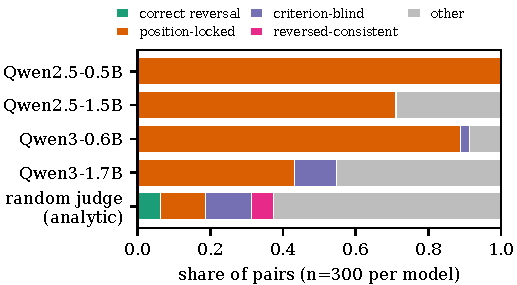
\includegraphics[width=\columnwidth]{figures/fig_taxonomy.pdf}
% Generated by make_figures.py from ../results/analysis.json.
\caption{Pair-level taxonomy shares (W1), n=300 pairs per judge, with the analytic random-judge reference.
Segments are stacked left to right in the legend order (correct reversal first). Correct reversal is
visible only as a 0.003-wide leftmost sliver for Qwen3-1.7B; the 0.062 leftmost segment of the random-judge
bar gives the scale.}
\label{fig:tax}
\end{figure}

\textbf{H2 (position-locking dominates): supported} for both pre-specified judges (Table~\ref{tab:hyp}).
For Qwen2.5-0.5B the result is degenerate: it answers ``A'' on all 1600 passes, so its row in
Table~\ref{tab:main} is identical to the always-A reference. Its H2 support therefore reflects a pure format
or letter-prior failure, not a property of the criterion. Qwen3-0.6B is less extreme (A on 1527 of 1600
passes) and still position-locked on 0.890 of non-correct-reversal pairs. In exploratory analysis, the larger
judge in each family is less position-locked (Qwen2.5-1.5B 0.710, Qwen3-1.7B 0.431), but the difference goes
into the ``other'' category (0.287 and 0.453) rather than into correct reversal.

\textbf{H1 (flip rate rises with size): inconclusive} under the pre-registered rule, because
$n_\mathrm{cond}$ is 0 for Qwen2.5-0.5B and 15 for Qwen3-0.6B. Descriptively, the Qwen3 conditional flip rate
moves from 0.000 to 0.008 (97.5\% CI of the difference [0.000, 0.030]); for Qwen2.5 it is undefined for the
small judge and 0.000 for the large one, so no bootstrap difference is defined. The chance-normalized
unconditional flip differences have 97.5\% CIs of [0.000, 0.040] (Qwen2.5) and [$-0.018$, 0.053] (Qwen3). All
quantities are near zero, so the data show no evidence of a size trend in this range; they equally cannot rule
out a trend at larger sizes.

\begin{table}[t]
\centering
% Source: ../results/analysis.md sections "H1" and "H2" == ../results/analysis.json (h1, models.*.h2_poslocked_share_ci95,
% models.*.pooled.pos_locked_share_of_noncr, n_noncr). Bootstrap: 2000 resamples of the 300 pooled pairs.
\caption{Hypothesis statistics (paired/percentile bootstrap, 2000 resamples over 300 pairs). H2 rows marked *
are exploratory (not pre-specified).}
\label{tab:hyp}
\resizebox{\columnwidth}{!}{%
\begin{tabular}{llr}
\toprule
\multicolumn{3}{l}{\textbf{H2}: position-locked share among non-correct-reversal pairs (95\% CI)} \\
Judge & $n$ & Share [CI] \\
\midrule
Qwen2.5-0.5B & 300 & 1.000 [1.000, 1.000] \\
Qwen3-0.6B & 300 & 0.890 [0.857, 0.927] \\
Qwen2.5-1.5B* & 300 & 0.710 [0.657, 0.763] \\
Qwen3-1.7B* & 299 & 0.431 [0.378, 0.487] \\
\midrule
\multicolumn{3}{l}{\textbf{H1}: cond.\ flip, large minus small (97.5\% CI); $n_\mathrm{cond}$ small/large} \\
Family & $n_\mathrm{cond}$ & Small $\to$ large [diff.\ CI] \\
\midrule
Qwen2.5 & 0 / 31 & undef.\ $\to$ 0.000 [undefined, 0 valid boots] \\
Qwen3 & 15 / 129 & 0.000 $\to$ 0.008 [0.000, 0.030] \\
\midrule
\multicolumn{3}{l}{Chance-normalized uncond.\ flip, large minus small (97.5\% CI)} \\
Qwen2.5 & 300 & [0.000, 0.040] \\
Qwen3 & 300 & [$-0.018$, 0.053] \\
\bottomrule
\end{tabular}}
\end{table}

\textbf{Controls (resample 0, 100 pairs, exploratory).} With the second negated wording W2 (``Which response
should be rejected?''), the correct-reversal share is 0.000 for all four judges (W1 on the same 100 pairs:
0.000, 0.000, 0.000, 0.010). In the length control, on the 72 pairs whose responses differ in character length,
the share of pairs where the longer response is picked in both orders is 0.000, 0.000, 0.014 and 0.250
(Qwen2.5-0.5B, Qwen2.5-1.5B, Qwen3-0.6B, Qwen3-1.7B). The random-judge level for this statistic is 0.25, so
no judge shows length sensitivity under this prompt. For the position-locked judges this control is
uninformative, since a judge that always emits the same letter cannot follow any criterion. For the two larger
judges it suggests (exploratory) that the reversal failure is not specific to negation. Scoring the length control by characters was not pre-registered.
% Source: ../results/analysis.md section "Secondary" == ../results/analysis.json (w2_r0, w2_r0_w1_same_pairs, length_ctrl).

\textbf{Letter use by criterion (exploratory).} Fig.~\ref{fig:letters} shows the share of passes answered
``A'' for each question, computed from the raw per-pass records. Qwen2.5-0.5B answers ``A'' to every question
and Qwen3-0.6B does so on 0.943 to 0.990 of passes. The two larger judges do change their output with the
question, but mostly as a shift in letter preference: Qwen2.5-1.5B answers ``A'' on 0.198 of \emph{better}
passes and 0.008 of W1 passes; Qwen3-1.7B on 0.338 and 0.115. A shift of the letter prior that does not depend
on which response sits behind the letter cannot produce correct reversals, which is consistent with the
near-zero correct-reversal shares. We did not pre-register this analysis and do not test it formally.
% Source: figures/paper_stats.json (letter_share_A), generated by make_figures.py from ../results/raw_*.json.

\begin{figure}[t]
\centering
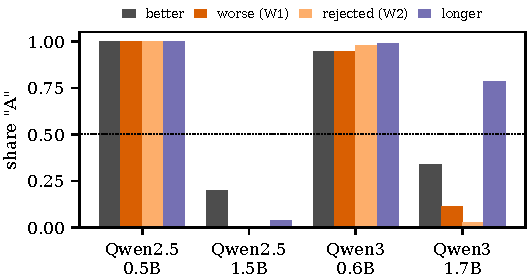
\includegraphics[width=\columnwidth]{figures/fig_letter_share.pdf}
% Generated by make_figures.py from ../results/raw_*.json.
\caption{Share of passes answered ``A'' per question (better and W1: 600 passes per judge; W2 and length: 200
passes, resample 0 only). Dotted line: 0.5.}
\label{fig:letters}
\end{figure}

\textbf{Per section.} Table~\ref{tab:sec} breaks results down by RewardBench section. The chat section has only
12 pairs because most chat responses exceed 150 tokens, and reasoning (code and math) dominates with 223 pairs,
so section differences should not be over-read. The only correct reversal (Qwen3-1.7B) is in chat-hard.

\begin{table}[t]
\centering
% Source: ../results/analysis.md section "Per section" == ../results/analysis.json (models.*.per_section).
\caption{Per-section results (W1). Acc.: position-consistent accuracy under ``better''. PL / CB / CR: shares of
position-locked, criterion-blind, correct-reversal pairs.}
\label{tab:sec}
\resizebox{\columnwidth}{!}{%
\begin{tabular}{llrrrrrr}
\toprule
Judge & Section & $n$ & Acc. & $n_\mathrm{cond}$ & PL & CB & CR \\
\midrule
Qwen2.5-0.5B & chat & 12 & 0.000 & 0 & 1.000 & 0.000 & 0.000 \\
 & chat-hard & 65 & 0.000 & 0 & 1.000 & 0.000 & 0.000 \\
 & reasoning & 223 & 0.000 & 0 & 1.000 & 0.000 & 0.000 \\
Qwen2.5-1.5B & chat & 12 & 0.083 & 1 & 0.917 & 0.000 & 0.000 \\
 & chat-hard & 65 & 0.092 & 6 & 0.862 & 0.000 & 0.000 \\
 & reasoning & 223 & 0.108 & 24 & 0.655 & 0.004 & 0.000 \\
Qwen3-0.6B & chat & 12 & 0.333 & 4 & 0.667 & 0.083 & 0.000 \\
 & chat-hard & 65 & 0.062 & 4 & 0.800 & 0.062 & 0.000 \\
 & reasoning & 223 & 0.031 & 7 & 0.928 & 0.009 & 0.000 \\
Qwen3-1.7B & chat & 12 & 0.667 & 8 & 0.000 & 0.417 & 0.000 \\
 & chat-hard & 65 & 0.369 & 24 & 0.215 & 0.169 & 0.015 \\
 & reasoning & 223 & 0.435 & 97 & 0.516 & 0.081 & 0.000 \\
\bottomrule
\end{tabular}}
\end{table}

\section{Discussion and Limitations}
\textbf{Interpretation.} The dominant failure in the smallest judges is position-locking, not
criterion-blindness: they emit the same letter whatever the question. This makes the negation test
uninformative about whether they ``understand'' negation. The larger judges do not ignore the question, but
they fail to condition on it in a content-appropriate way. Qwen3-1.7B shows content dependence under
\emph{better}: its position-consistent accuracy of 0.430 is above the 0.25 ceiling of a judge driven by
letter preference alone, yet it does not reverse under W1. That the W1 response is mainly a shift in letter
preference (Fig.~\ref{fig:letters}) is a hypothesis consistent with the data, not a formally tested
finding. For practitioners, the
consequence is that sub-2B judges in this configuration should not be trusted to follow the stated criterion;
order-swapped and criterion-negated checks are cheap and expose this immediately.

\textbf{Threats to validity.}
(i)~\emph{Scope}: four Qwen models up to 1.7B, one benchmark, one prompt template; no 3B+ judge was run, and
larger or reasoning-enabled judges may behave differently. Prior work reports that thinking mode improves small
Qwen3 judges on RewardBench~\cite{jayarao2025explicit}; we disabled it.
(ii)~\emph{Readout}: the A-vs-B logit comparison without generation can disagree with what the model would
generate. Qwen3-1.7B has a mean A/B mass of 0.745, and 25.2\% of its \emph{better}/W1 passes have mass below 0.5
(Qwen3-0.6B: 1.7\%; the Qwen2.5 judges: 0), so its letter comparison is less clean.
(iii)~\emph{Data filter}: keeping responses of at most 150 tokens and prompts of at most 400 tokens biases the
sample toward short code and math items (reasoning is 223 of 300 pairs).
(iv)~\emph{Strict scoring}: position-consistent accuracy requires correctness in both orders, so low accuracy
reflects weak judges, not necessarily harm from the prompt.
(v)~\emph{Prompts}: one pass per prompt and no wording search beyond W1/W2; conclusions are about these prompts.
(vi)~\emph{Statistics}: H1 could not be evaluated as designed because the conditioning subsets are tiny; the
exploratory H2 values for the larger judges and the character-based length scoring were not pre-registered;
the development-set A/B-mass exclusion check was run for Qwen2.5-0.5B only (20 pairs), not for the other three
judges (protocol deviation; all four have evaluation-set mean mass $\ge 0.745$).
(vii)~\emph{Novelty}: the related-work scan used arXiv and web search only.

\textbf{What did not work.} The pre-registered size comparison (H1) did not yield a usable test, because the
competence condition it relies on (correct under ``better'' in both orders) is almost never met by the smallest
judges. A design that conditions on single-order correctness, or uses stronger judges, would be needed to
measure a flip-rate trend.

\section{Conclusion}
Asked ``which response is worse?'', four open Qwen judges between 0.5B and 1.7B parameters almost never reverse
their ``better'' verdict correctly (0, 0, 0 and 1 of 300 RewardBench pairs). The two smallest are dominated by
position-locking (H2 supported, in one case trivially, as an always-A judge); the size-trend hypothesis (H1) is
inconclusive. The larger judges change their output with the question but fail to condition on it in a
content-appropriate way: Qwen3-1.7B is above the letter-preference ceiling under ``better'' (0.430 vs.\ 0.25)
yet does not reverse under ``worse''. Exploratory ``which is longer?'' controls are also not followed. Whether criterion reversal emerges at 3B+ parameters, with thinking enabled, or under
generated rather than logit-read verdicts is left open.

\section*{Reproducibility Statement}
Repository path: \url{projects/small-judge-reversal/}. Raw per-pass outputs are committed in
\url{results/raw_<model>_r<k>.json}; model and data revisions in \url{results/models.md}; the
environment in \url{results/pip_freeze.txt}; exact commands in \url{results/commands.md}. From the project
directory:
{\footnotesize
\begin{verbatim}
uv venv .venv --python 3.14
uv pip install --python .venv/bin/python \
  -r requirements.txt
./fetch_data.sh
OMP_NUM_THREADS=4 .venv/bin/python -I \
  src/run.py prepare
# for M in the 4 models, s in 0 1 2:
OMP_NUM_THREADS=4 .venv/bin/python -I \
  src/run.py run --model $M --resample $s
.venv/bin/python -I src/analyze.py
python -I paper/make_figures.py # needs matplotlib
\end{verbatim}}
Only \texttt{src/analyze.py} and \texttt{paper/make\_figures.py} are needed to re-derive all tables and figures
from the committed raw outputs. Re-running inference took 2.37 h of summed forward time at 4 threads (about 4 h wall-clock per \texttt{README.md}).

\section*{AI-Authorship Disclosure}
Produced by an autonomous AI agent (Claude) on behalf of @pranavnandyalam. Not peer reviewed. The study design,
code, experiments, analysis and this text were produced by the agent; the plan and results were reviewed by
automated overseer and ethics agents, not by human peer review.

\bibliographystyle{IEEEtran}
\bibliography{refs}

\end{document}
